\subsection{Testing plan}
%%\includegraphics[scale=0.8] {Testing_Plan.pdf}
The testing approach for our project is using the bottom-up methodology. Each member of group 2 will be responsibility for their own tests. After finishing their own tests, they need to report to the test manager and then the test manager will carry out the system integration test. The responsibility of each member will be presented in the following part. The tool for testing is JUnit, which is used to check whether it has a bug in the whole program. The test will distribute into 3 levels:
\begin{itemize}
\item Functional Level
\item Integration Level
\item User Level
\end{itemize}
\textbf{Functional Testing:} Each member in group 2 will be assigned to a part of program, which contains a complete function in the robot. To ensure the quality of testing, each member must create sufficient white-box tests and report the test cases with test results to the test manager. It is recommended to swap the task of testing with other team members to let them test your code.
\\
\newline
\textbf{Component Test:} 
This test is to isolate the different components from each other to test and verify the correctness between components. The components are divided in following:
\\	
	\\-AI, responded by Matthew Nestor and Bowen Tao
	\\-GUI and Map Editor, responded by Yifei Pei and Jianqiu Li
	\\-Communication, responded by Abdulaziz Alhulayfi and Yu Hong
\\
\newline
\textbf{Integration Testing:}
The integration test is using bottom-up approach to test the correctness of the whole program. Simultaneously this test also should test whether it has exceptions and errors.  
\\
\newline
\textbf{Regression Test:} 
This test is to keep the system stable. After a bug is fixed, we must make sure that the original system function performs correctly. So a regression test is needed.
\\
\newline
\textbf{Stress Test:} 
It is used to test the robustness of the whole program when the data is flooding. Especially, in terms of the sensor receiver and communication, they should be tested thoroughly.
\\
\newline
\textbf{Final Test:} 
All the bugs which is found in the former tests will need to be fixed, to ensure that the whole program could run correctly.  

\subsection{Test Document}
Every group member will write a test report and submit to the test manager and a combined test report will be present in LaTex format.


\subsection{Quality Assurance Plan}

\begin{center}
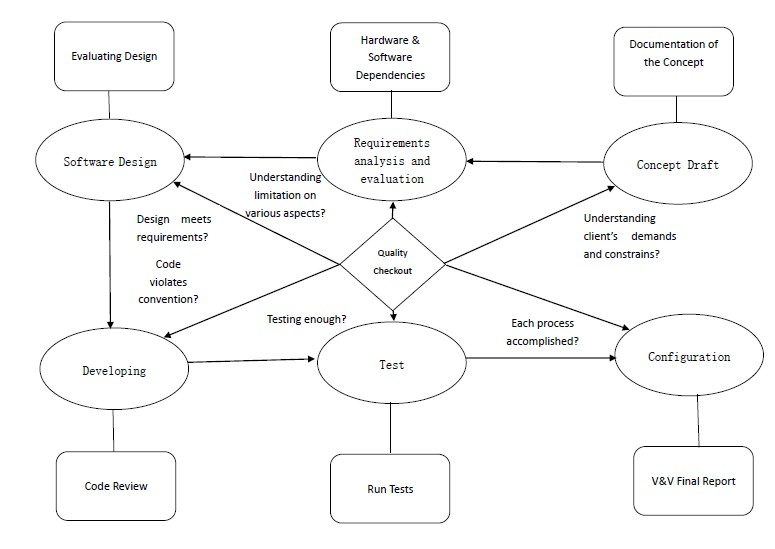
\includegraphics[scale=0.5]{images/image.jpg}
\end{center}
\begin{center}
\item {Diagram 3: Quality Assurance plan}
\end{center}
Quality Assurance Plan provides a guide line for each developer to assess the deliverables' quality in each process. It handles the life cycle in development to satisfy the established SRS.    
\subsection{Verification \& Validation Process}
\subsubsection{One more thing}
The PMBOK guide is defined as follows in its 4th edition:
"Validation. The assurance that a product, service, or system meets the needs of the customer and other identified stakeholders. It often involves acceptance and suitability with external customers. Contrast with verification."\\
"Verification. The evaluation of whether or not a product, service, or system complies with a regulation, requirement, specification, or imposed condition. It is often an internal process. Contrast with validation."
\subsection{Verification \& Validation Procedures}
\newpage
\rowcolors{1}{lightgray}{white}
\begin{center}
\begin{tabular}{p{4.0cm} |p{3.5cm}|p{5cm} |}
\hline
Phase & Tasks&Key Issues \\
1.Concept Draft & Conceptual documentation	& Absorbing and understanding user's demands and discussing the constrains of implementation.\\
2. Requirements analysis and evaluation & & Analysing requirements and evaluate feasibility\\
3. Software Design & 1. Maintainability: Coding convention and documentation \newline
2. Safety evaluation \newline
3. Design analysis \newline
4. Interface design \newline
5. Stress analysis \newline
6. Test design \newline
1. & Make a rule for coding and commentating.\newline
2. Evaluating potential risk in the robot project.\newline
3. Design architecture of the robot project based on analysed requirement.\newline
4. The interface correctness, reliability and completeness in terms of hardware, software and user.\newline
5. Analysis the extreme situation in the robot project\newline
6. Design test cases \\
4. Developing 
&1. Coding based on analysis and design above\newline
2. Run functional and component tests\newline
 &1. Ensure the quality of the codes and member contribution.\newline
2. Submit test cases with results.\newline
5. Test &1. Run integration test\newline
2. Run regression test\newline
3. Run stress test\newline
4. Run final test\newline
 & 1. Submit the test cases with results.\newline
2.Submit the test cases with results.\newline
3. Submit the test cases with results.\newline
4. Ensure all bugs are fixed and the stability of the whole program\\
6. Configuration
&1. Configurable auditing\newline
2. V\&V final report\newline 
3. Test report


 
\end{tabular}
\end{center}
\begin{center}
\item {Table: V\&V Procedure}
\end{center}
\newpage


\section{Attachment: QA Check-list}
\subsection{Objective}

To check the quality of software development in different phases which contain the V\&V processes. This check-list will provide a intuitionistic feedback in terms of the software development, using by the score of the validation questions:\\

\subsection{Structure \& Assessment}

The document will be used to perform the checkout of quality, but considering the time allowed for the project, we will just hold the assessment twice.  
The first assessment date will be between the mid-break (21st Sep 2013 - 7th Oct 2013) and the second one will be held on Week 12 (28th Oct 2013 to 1 Nov 2013), which will be before the final presentation. Specific date will be negotiated by the group members within the period.\\
The evaluation way is defined: If Y is ticked then the marks will be increased by 1 whist N is ticked then the marks will be increased by 0. And if NA is ticked then the marks will be increased by -1.\\
The higher marks we get, the higher quality of the software development. 
\newline
   




\newpage
\subsection{Concept and Draft}
Date Performed: 
\\Performed by: 
\\Comments:
\begin{center}
\rowcolors{1}{lightgray}{white}

    \begin{tabular}{p{0.5cm} |  p{3.5cm} |  p{0.5cm} |p{0.5cm} |p{0.5cm} | p{5cm} |}
    \hline

    Item No.& Validation Item &Y &N &NA & Comment \\ \hline\hline
	3.1 &
	Does all group member understand the requirement which is proposed by the client?&
	$\text{\rlap{}}\square$& 
	$\text{\rlap{}}\square$&
	$\text{\rlap{}}\square$&
 \\ \hline


    3.2 &
	Is the requirements possible to translate into code?&
	$\text{\rlap{}}\square$& 
	$\text{\rlap{}}\square$&
	$\text{\rlap{}}\square$& \\ \hline


    3.3& 
	Has the requirements been recorded and translated into the document?&
	$\text{\rlap{}}\square$& 
	$\text{\rlap{}}\square$&
	$\text{\rlap{}}\square$& 
	\\ \hline


    3.4 &
	Has the development used a software model and software processes?&
	$\text{\rlap{}}\square$& 
	$\text{\rlap{}}\square$&
	$\text{\rlap{}}\square$& \\ \hline
	
    \end{tabular}
\end{center}



\newpage


\subsection{Requirement Analysis and Evaluation}
Date Performed:
\\Performed by:
\\Comments:

\begin{center}
\rowcolors{1}{lightgray}{white}

    \begin{tabular}{p{0.5cm} |  p{3.5cm} |  p{0.5cm} |p{0.5cm} |p{0.5cm} | p{5cm} |}
    \hline
	Item No.& Validation Item &Y &N &NA & Comment \\ \hline\hline

    	4.1 &
	Does the SRS has a clear structure so that the client could be easy to understand?&
	$\text{\rlap{}}\square$&
	$\text{\rlap{}}\square$&
	$\text{\rlap{}}\square$& \\ \hline

    4.2& 
	Has the SRS been presented to the client?&
	$\text{\rlap{}}\square$&
	$\text{\rlap{}}\square$&
	$\text{\rlap{}}\square$& \\ \hline

    4.3 &
	Has the group discussed with the client when there are changes in SRS?&
	$\text{\rlap{}}\square$&
	$\text{\rlap{}}\square$&
	$\text{\rlap{}}\square$& \\ \hline
	

    4.4 &
	Have the changes of requirements been documented in SRS?&
	$\text{\rlap{}}\square$&
	$\text{\rlap{}}\square$&
	$\text{\rlap{}}\square$& \\ \hline

    4.5&
	Have the tasks been allocated and explained clearly to the group members?&
	$\text{\rlap{}}\square$&
	$\text{\rlap{}}\square$&
	$\text{\rlap{}}\square$& \\ \hline

    4.6&
	Has the group evaluate the risk of the whole project?&
	$\text{\rlap{}}\square$&
	$\text{\rlap{}}\square$&
	$\text{\rlap{}}\square$& \\ \hline
    \end{tabular}
\end{center}





\newpage
\subsection{Software Design}
Date Performed:
\\Performed by:



\begin{center}
\rowcolors{1}{lightgray}{white}

    \begin{tabular}{p{0.5cm} |  p{3.5cm} |  p{0.5cm} |p{0.5cm} |p{0.5cm} | p{5cm} |}
    \hline
	Item No.& Validation Item &Y &N &NA & Comment \\ \hline\hline
	

    5.1&
	Has the precautions been taken to prevent the chaos of the data type?&
	$\text{\rlap{}}\square$&
	$\text{\rlap{}}\square$&
	$\text{\rlap{}}\square$& \\ \hline

    5.2&
	Has a safety analysis been adopted in the design?&
	$\text{\rlap{}}\square$&
	$\text{\rlap{}}\square$&
	$\text{\rlap{}}\square$& \\ \hline

    5.3&
	Has the system design been presented clearly to the group member?&
	$\text{\rlap{}}\square$&
	$\text{\rlap{}}\square$&
	$\text{\rlap{}}\square$& \\ \hline
 

    5.4&
	Has hardware limitation been taken account of when the system designs?&
	$\text{\rlap{}}\square$&
	$\text{\rlap{}}\square$&
	$\text{\rlap{}}\square$& \\ \hline
 

    5.5&
	Have the majority of potential risks been avoided by the design?&
	$\text{\rlap{}}\square$&
	$\text{\rlap{}}\square$&
	$\text{\rlap{}}\square$& \\ \hline
 

    5.6&
	Have the code convention, developing tools and testing tools been unified?&
	$\text{\rlap{}}\square$&
	$\text{\rlap{}}\square$&
	$\text{\rlap{}}\square$& \\ \hline


 


 
    \end{tabular}
\end{center}



\newpage
\subsection{Developing}
Date Performed:
\\Performed by:


\begin{center}
\rowcolors{1}{lightgray}{white}

    \begin{tabular}{p{0.5cm} |  p{3.5cm} |  p{0.5cm} |p{0.5cm} |p{0.5cm} | p{5cm} |}
    \hline
	Item No.& Validation Item &Y &N &NA & Comment \\ \hline\hline
	

    6.1&
	Have special/additional requirements been documented?& 
	$\text{\rlap{}}\square$&  
	$\text{\rlap{}}\square$&
	$\text{\rlap{}}\square$& 
	\\ \hline

    6.2&
	Does all code have adequate comments so that it is easy to read by each member in the group?&
	$\text{\rlap{}}\square$&
	$\text{\rlap{}}\square$&
	$\text{\rlap{}}\square$& 
	\\ \hline

    6.3&
	Has the code review session been held?&
	$\text{\rlap{}}\square$&
	$\text{\rlap{}}\square$&
	$\text{\rlap{}}\square$&
\\ \hline

    6.4&
	Have all group members clearly know the code tasks?&
	$\text{\rlap{}}\square$&
	$\text{\rlap{}}\square$&
	$\text{\rlap{}}\square$& 
	\\ \hline

    6.5&
	Does each function have its own succinct description?&
	$\text{\rlap{}}\square$&
	$\text{\rlap{}}\square$&
	$\text{\rlap{}}\square$& 
	\\ \hline

    6.6&
	Have the white-box tests been created and reported the results to the test manager?&
	$\text{\rlap{}}\square$&
	$\text{\rlap{}}\square$&
	$\text{\rlap{}}\square$& 
	\\ \hline

    6.7&
	Did the whole program pass all functional and component tests?&
	$\text{\rlap{}}\square$&
	$\text{\rlap{}}\square$&
	$\text{\rlap{}}\square$& 
	\\ \hlineteam 

    6.8&
	Has test report included all the test results?&
	$\text{\rlap{}}\square$&
	$\text{\rlap{}}\square$&
	$\text{\rlap{}}\square$& 
	\\ \hline
	
 	6.9&
	Has the client been told when the SRS has been updated?&
	$\text{\rlap{}}\square$&
	$\text{\rlap{}}\square$&
	$\text{\rlap{}}\square$& 
	\\ \hline

   
    \end{tabular}
\end{center}



\newpage
\subsection{Testing}
Date Performed:
\\Performed by:



\begin{center}
\rowcolors{1}{lightgray}{white}

    \begin{tabular}{p{0.5cm} |  p{3.5cm} |  p{0.5cm} |p{0.5cm} |p{0.5cm} | p{5cm} |}
    \hline
	Item No.& Validation Item &Y &N &NA & Comment \\ \hline\hline
	

    7.1&
	Is there any mirror bug affecting the whole program?&
	$\text{\rlap{}}\square$&
	$\text{\rlap{}}\square$&
	$\text{\rlap{}}\square$& \\ \hline

    7.2&
	Are the error messages kept independently?&
	$\text{\rlap{}}\square$&
	$\text{\rlap{}}\square$&
	$\text{\rlap{}}\square$& \\ \hline

    7.3&
	Are all errors during the testing been recorded?&
	$\text{\rlap{}}\square$&
	$\text{\rlap{}}\square$&
	$\text{\rlap{}}\square$& \\ \hline
 

    7.4&
	Did the whole program pass all integration tests?&
	$\text{\rlap{}}\square$&
	$\text{\rlap{}}\square$&
	$\text{\rlap{}}\square$& \\ \hline
  

    7.5&
	Did the whole program pass all regression and stress tests?&
	$\text{\rlap{}}\square$&
	$\text{\rlap{}}\square$&
	$\text{\rlap{}}\square$& \\ \hline
  

    7.6&
	Did the whole program pass final test?&
	$\text{\rlap{}}\square$&
	$\text{\rlap{}}\square$&
	$\text{\rlap{}}\square$& \\ \hline
   
 
    \end{tabular}
\end{center}
